\begin{figure}[tb]
\centering
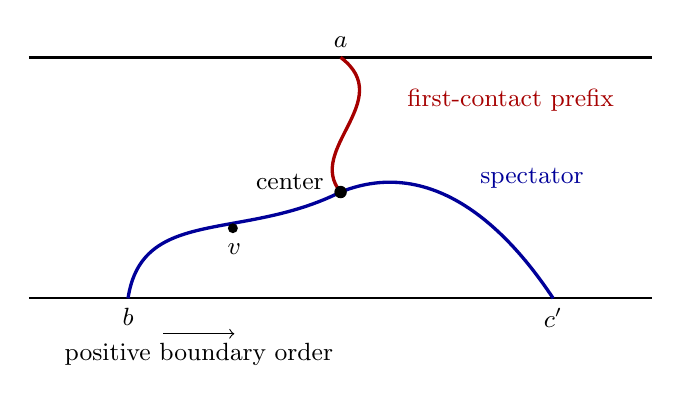
\begin{tikzpicture}[scale=.9, every node/.style={font=\small}]
 \draw[thick] (-.4,0)--(8.4,0);
 \draw[thick] (-.4,3.4)--(8.4,3.4);
 \node[below] at (1,0) {$b$};
 \node[below] at (7,0) {$c'$};
 \node[above] at (4,3.4) {$a$};
 \draw[very thick,blue!60!black] (1,0)
  .. controls (1.2,1.3) and (2.6,.8) .. (4,1.5);
 \draw[very thick,blue!60!black] (4,1.5)
  .. controls (5.5,2.1) and (6.6,.6) .. (7,0);
 \draw[very thick,red!65!black] (4,3.4)
  .. controls (4.8,2.8) and (3.5,2.1) .. (4,1.5);
 \fill (4,1.5) circle (2.5pt);
 \node[left] at (3.9,1.65) {center};
 \fill (2.48,.99) circle (2pt);
 \node[below] at (2.5,.91) {$v$};
 \node[blue!60!black] at (6.7,1.7) {spectator};
 \node[red!65!black] at (6.4,2.8) {first-contact prefix};
 \draw[->] (1.5,-.5)--(2.5,-.5);
 \node[below] at (2,-.5) {positive boundary order};
\end{tikzpicture}
\caption{A contact tripod, shown schematically. The arch from $b$ to
$c'$ is the spectator and a prefix from the opposite port $a$ reaches
it for the first time at the center. The center is weighted once.
Reassigning the active arm gives the two bridge-spectator terms.
The vertex $v$ may lie on any arm or at the center; the restrictions
in the proof keep these cases separate.}
\label{fig:pv:tripod}
\end{figure}
